\section{Project Description}
\label{sec:desc}

\noindent
We propose to hold a symposium with a novel format which brings
together a small ($\sim 30$ people) yet highly motivated group of
experts focusing on smarter methods in ocean observation.

\begin{wrapfigure}{!h}{2.8in}
  \vspace{-0.5cm}
  \centering 
  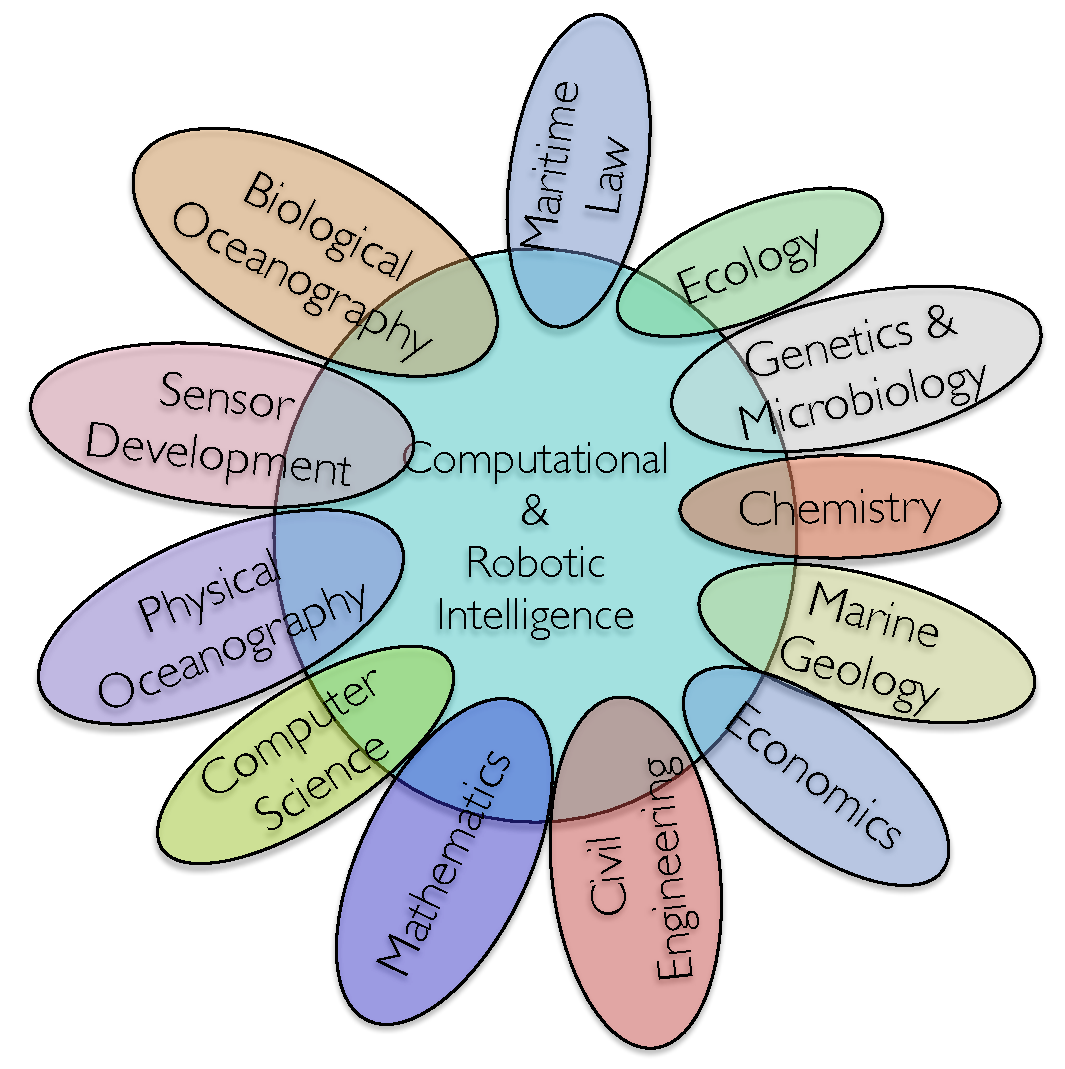
\includegraphics[scale=0.4]{fig/disciplines.pdf}
  \caption{The expectation of multi-disciplinary presentations for the
    \sympe. Given the intimate nature of the event, not all these
    fields would likely be represented.}
  \label{fig:concept}
  \vspace{-0.5cm}
\end{wrapfigure}

Our primary aim of this symposium is to generate ideas across science
and technology with a central focus on computational and robotic
intelligence (Fig. \ref{fig:concept}).  In the process, we hope to
make connections for ideation to advance observation methods at
various levels (national, international), during this \textsf{UN
  Decade of the Oceans}~\footnote{\url{https://oceandecade.org/}}. By
doing so, we hope for scientists to understand and leverage advances
in technology and for technologists to advance their science and
problem solving methods to have a real societal impact. And together,
to advance the state of ocean science and our understanding of the
world's ocean.

While there is a general acceptance of the need for inter-disciplinary
efforts in the field and out of it, expertise continues to be siloed
and researchers tend to focus narrowly, missing out on integrative and
potentially more expansive efforts. This meeting is an attempt to
bringing people together in meaningful debate and interaction across
disciplinary, geographic and cultural boundaries, and do so in an
immersive, safe and thoughtful environment, where reaching out can
provide research dividends.

By interaction across disciplines, we imply those which ought to
occur, but rarely do. Our proposed \emph{by invitation only} symposium
aims to be different and meaningful in a number of ways:

\begin{itemize}

\item We expect people to present speculative and ``far-out'' yet
  grounded ideas/hypotheses/concepts which commingle with
  inter-disciplinary concepts, processes and actions. So for example,
  a biological oceanographer, speculating what it might take to get a
  measure of biodiversity within a volume of water, and how it might
  evolve with environmental variability. Or a roboticist trying to
  advance the state of online machine learning for a mobile platform
  to take measure of planktonic community structure using in-situ
  machine vision, as an example. 

\item We will pair each speaker with a 'commentator/critic' from a
  very different field who would be expected to reach into the
  speaker's ideas, shared \emph{a priori} to provide public feedback
  during the event. 

\item This is \emph{not} a talk-and-drop event, but participatory by
  design. So each participant will not only have an opportunity to
  present, but also play critic to someone else. This also means the
  pace of the \symp will be more deliberate with adequate time for
  discussions, debates and networking, across \textbf{4 days}
  including (potentially) two half days around a social/outdoor
  activity (see Table \ref{tab:symp}). The final schedule will be
  outlined when we have a quorum of invitees.

\end{itemize}  

\noindent
Such approaches in interaction, have long been used in Cognitive
Science and applied by one of us (Rajan) when founding the \nas
Workshop of Planning and Scheduling (a niche sub-discipline within
AI). Panels and posters will be part of the program but the critical
nature of open interaction makes for a kind of back-and-forth that
cannot be preordained or scripted. And if designed properly, this can
lead to a truly interactive and participatory process. We have also
successfully used this approach in the maritime community in 2013 in
Gran Canaria and a symposia in Trondheim in 2018, which while
participatory, was not as direct as what we're proposing here. The
more deliberative aspects of this proposed event are seeded in early
Computer Science conferences in the late 60's and 70's in Asilomar,
California as also the 'Gordon Research Conferences' in the sciences,
albeit in a more intimate environment.

The symposium has already been endorsed by the UN Decade of the Ocean
committee. The symposium website reflects this endorsement, which has
been important in being able to reach out to the scientific community
as also in the context of recruiting early stage researcher
participation.
